\section{Simulation}

% \begin{frame}{Simulation Background}
%     \framesubtitle{What are we simulating?}

%     \begin{wideitemize}
%         \item The simulation is based my CS257 coursework submission \parencite{modules:aca257submission}.
%         \begin{wideitemize}
%             \item Optimized for SIMD processing, embarassingly parallel.
%         \end{wideitemize}
%         \item The original CS257 code was taken from \parencite{book:griebel1998numerical}.
%         \item 2D Simulation of ``laminar flows of viscous, incompressible fluids''.
%     \end{wideitemize}
% \end{frame}

\begin{frame}{Simulation Background}
    \framesubtitle{What are we simulating?}
    
    \begin{columns}[t, onlytextwidth]
        \begin{column}{0.7\textwidth}
            \begin{wideitemize}
                \item The simulation is based on my CS257 coursework submission \parencite{modules:aca257submission}.
                \begin{wideitemize}
                    \item Optimized for SIMD processing, embarassingly parallel.
                \end{wideitemize}
                \item The original CS257 code was taken from \parencite{book:griebel1998numerical}.
                \item 2D Simulation of ``laminar flows of viscous, incompressible fluids''.
                \begin{wideitemize}
                    \item Laminar flow $\rightarrow$ Fluid moves in layers (the opposite of turbulent flow).
                    \item Viscous $\rightarrow$ High internal friction forces.
                    \item Incompressible $\rightarrow$ Fluid density is constant throughout.
                \end{wideitemize}
                \item Simulation calculates {2D velocity $u,v$ and pressure $p$}.
            \end{wideitemize}
        \end{column} 
        \begin{column}{0.3\textwidth}
            \begin{figure}
                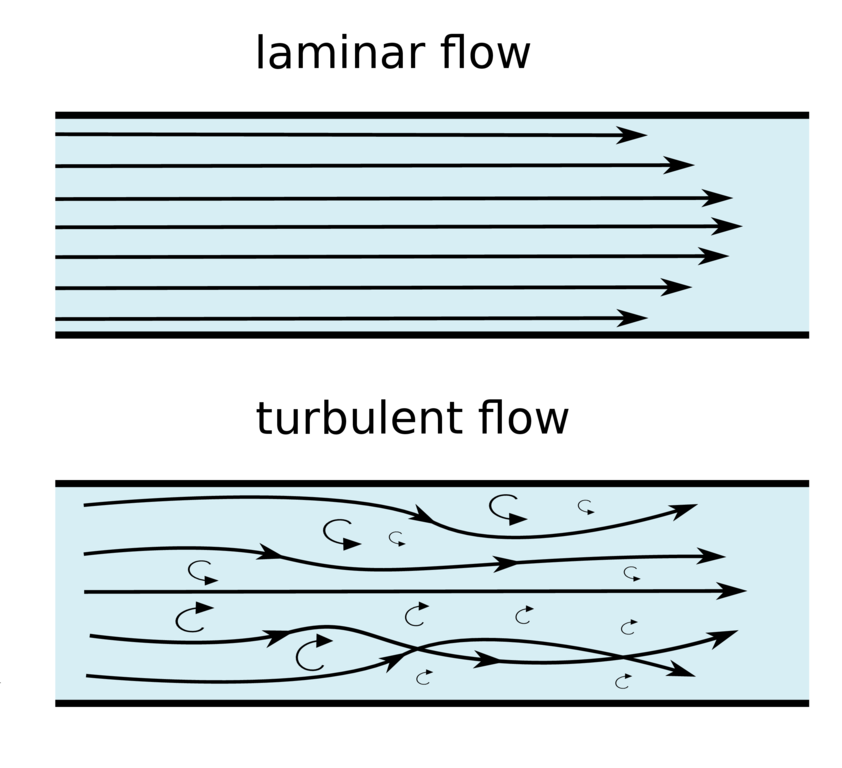
\includegraphics[width=\textwidth]{Presentation/images/sketch-laminar-flow-turbulent-flow.png}
                \caption{Laminar vs. turbulent fluid flow. Reproduced from cfdsupport.com}
                \label{fig:laminar_flow}
            \end{figure}
        \end{column}
    \end{columns}
\end{frame}

\begin{frame}{Simulation Variables}
    \framesubtitle{What are we simulating?}
    \begin{wideitemize}
        \item Fluid flows in from the left at $\SI{1}{\metre\per\second}$.
        \item Fluid viscosity controlled by the Reynolds number $Re$  \parencite{falkovich2018fluid}.
        \item These and other simulation parameters are kept equal to the CS257 coursework. 
    \end{wideitemize}
    
    \todomark{Visualization here}
\end{frame}

\begin{frame}{Simulation Method}
    \framesubtitle{How do we simulate it?}
    
    \begin{wideitemize}
        \item Majority of sim time spent solving the Poisson equation for $p$.
        \item Uses an iterative solver.
        \item Iteration count fixed at 100 for the ACA coursework\footnote{A more accurate simulation would calculate until the difference is within a tolerance value}.
        \item Equation is solved once per tick (timestep depends on fluid velocity).
    \end{wideitemize}
    
    \ddef{Poisson Equation}{
        \begin{equation*}
            \frac{\partial^2{p^{(n+1)}}}{\partial{x^2}} + \frac{\partial^2{p^{(n+1)}}}{\partial{y^2}} =  \frac{1}{\delta{t}}\left(\frac{\partial{f^{(n)}_{i,j}}}{\partial{x}} + \frac{\partial{g^{(n)}_{i,j}}}{\partial{y}}\right)
        \end{equation*}
    }
\end{frame}

\begin{frame}{Simulation Method}
    \framesubtitle{How do we simulate it?}
    
    \begin{wideitemize}
        \item Majority of sim time spent solving the Poisson equation for $p$.
        \item Uses an iterative solver.
        \item Iteration count fixed at 100 for the ACA coursework\footnote{A more accurate simulation would calculate until the difference is within a tolerance value}.
        \item Equation is solved once per tick (timestep depends on fluid velocity).
    \end{wideitemize}
    \vspace{1em}
    
    \begin{adjustbox}{center}    
    \begin{tikzpicture}[
circlenode/.style={circle,fill=black,inner sep=0pt,minimum size=3pt,},
]
\def\scale{3.5}
    \draw[->] (0,0) node[circlenode,label=left:{$t$}](a){} -- (1*\scale, 0) node[circlenode,label=above:{$0.1$}](b){} -- (2.7*\scale,0) node[circlenode,label=above:{$0.27$}](c){} -- (3.2*\scale,0) node[circlenode,label=above:{$0.32$}](d){} -- (3.4*\scale,0);
    
    % from latexdraw.com
    \draw[|-|] ($ (a) + (0.1,-0.5) $) -- ($ (b) + (-0.1,-0.5) $) 
        node [midway, above]{$\delta{t} = 0.1$}
        node [midway, below]{100 iters};
        
    \draw[|-|] ($ (b) + (0.1,-0.5) $) -- ($ (c) + (-0.1,-0.5) $) 
        node [midway, above]{$\delta{t} = 0.17$}
        node [midway, below]{100 iters};
    
    \draw[|-|] ($ (c) + (0.1,-0.5) $) -- ($ (d) + (-0.1,-0.5) $) 
        node [midway, above]{$\delta{t} = 0.05$}
        node [midway, below]{100 iters};
        
    \end{tikzpicture}
    \end{adjustbox}
\end{frame}

% Centers around Poisson differential eq, solved iteratively
% Parameters such as Reynolds number, timestep safety, iteration count taken from ACA.
% Timing defined in terms of timesteps - upper bound defined based on security
% Fluid flows in from the left at a fixed velocity of 1m/s
